\section{Vorbereitung}

Die Vorbereitungsphase umfasst größtenteils die Portierung der
Steuerungssoftware von Micro-ROS auf FreeRTOS: Der Datenaustausch erfolgt intern
über FreeRTOS-Queues, während die Inter-Task-Synchronisation auf den
leichtgewichtigen Direct-Task-Notifications basiert. Zusätzlich wird die Methode
zur Sollgeschwindigkeitseingabe per UART mit CRC-Überprüfung implementiert. Den
Abschluss bildet die Aktivierung der Caches. Die Details zu den genannten
Maßnahmen folgen in den nächsten Abschnitten.

\subsection{Umstellung auf FreeRTOS}

\subsubsection{Übertragung von Sollgeschwindigkeiten}

In der bisherigen Implementierung erhielt der Mikrocontroller als Client
Geschwindigkeitssollwerte über das ROS2-Framework vom Micro-ROS-Agent auf einem
Linux-Host. Da Micro-ROS und damit die Kompatibilität mit ROS2-Framework
beseitigt wird, muss die Übertragung nun manuell realisiert werden.

Dazu wird zunächst eine Struktur \mintinline{cpp}|Vel2d| definiert, der die
2D-Geschwindigkeitswerte bündelt, welche vom Host an den Mikrocontroller
gesendet werden.

\begin{code}
\begin{minted}{cpp}
struct Vel2d {
  double x;
  double y;
  double z;
};
\end{minted}
    \captionof{listing}{Definition der Struktur für die Sollgeschwindigkeit}
\end{code}

Darauf aufbauend wird eine weitere Struktur \mintinline{cpp}|Vel2dFrame|
definiert, die als UART-Daten-Frame dient. Sie enthält nur zusätzlich ein Feld
\mintinline{cpp}|crc| für die CRC-Überprüfung und eine Methode
\mintinline{cpp}|compare()|, die einen nachträglich zu berechnenden CRC-Wert als
Parameter übernimmt und mit dem vorhandenen vergleicht. Durch das Attribut
\mintinline{cpp}|packed| wird verhindert, dass zusätzliches Padding für die
Speicherausrichtung eingefügt wird.

\begin{code}
\begin{minted}{cpp}
struct Vel2dFrame {
  Vel2d vel;
  uint32_t crc;

  bool compare(uint32_t rhs) { return crc == rhs; }
} __attribute__((packed));
\end{minted}
    \captionof{listing}{Definition des UART-Daten-Frames}
\end{code}

Für die Übertragung über UART wird die Funktion
\mintinline{cpp}|HAL_UARTEx_ReceiveToIdle_IT()| verwendet, um die serialisierten
Bytes eines Daten-Frames mittels der STM32-HAL in einen statisch vorallokierten
Puffer zu empfangen.

Dies ist gepaart mit einem Interrupt-Callback
\mintinline{cpp}|HAL_UARTEx_RxEventCallback()|, die entweder ausgelöst wird,
wenn -- wie der Name der assoziierten Übertragungsfunktion andeuten lässt -- die
HAL feststellt, dass die UART-Leitung nach einer Übertragung bereits für eine
bestimmte Zeit inaktiv ist (Idle-Zustand), oder wenn der Puffer einmal komplett
voll beschrieben wird~\cite{HAL_UARTEx_ReceiveToIdle_IT}. Der zweite Parameter
dieses Interrupt-Callbacks gibt immer die Größe der aktuell in den Puffer
geschriebenen Daten an.

\begin{code}
\begin{minted}{cpp}
// preallocated buffer with the exact size of a data frame
static uint8_t uart_rx_buf[VEL2D_FRAME_LEN];
volatile static uint16_t rx_len;

void HAL_UARTEx_RxEventCallback(UART_HandleTypeDef* huart, uint16_t size) {
  if (huart->Instance != huart3.Instance) return;

  rx_len = size;

  // unblock the task
  static BaseType_t xHigherPriorityTaskWoken;
  vTaskNotifyGiveFromISR(task_handle, &xHigherPriorityTaskWoken);
  portYIELD_FROM_ISR(xHigherPriorityTaskWoken);

  // reset reception from UART
  HAL_UARTEx_ReceiveToIdle_IT(&huart3, uart_rx_buf, sizeof(uart_rx_buf));
}

// setup reception from UART in task init
HAL_UARTEx_ReceiveToIdle_IT(&huart3, uart_rx_buf, sizeof(uart_rx_buf));
\end{minted}
    \captionof{listing}{Datenempfang über UART via Interrupt}
    \label{code:uart_isr}
\end{code}

Mit diesem Setup kann der Mikrocontroller nun Bytes direkt von einem Linux-Host
über UART empfangen. Die CRC-Prüfung kombiniert mit dem Idle/Timeout-Feature
gewährleisten einen fehlertoleranten Datenempfang.

Um die empfangenen Bytes zu parsen, ohne dies aber während der Ausführung des
Interrupt-Callbacks zu tun, wird eine eigenständige FreeRTOS-Task erstellt.
Mittels \mintinline{cpp}|vTaskNotifyGiveFromISR()| -- aufgerufen innerhalb des
Interrupt-Callbacks -- wird dieser Task signalisiert (\ref{code:uart_isr},
\ref{sec:direct_task_notification}). Demnach werden die empfangenen Bytes durch
\mintinline{cpp}|reinterpret_cast| zurück in ein Daten-Frame deserialisiert.

Folglich lässt sich zur Kontrolle ein CRC-Wert lokal aus den empfangenen
Geschwindigkeitswerten berechnen und mit dem empfangenen vergleichen. Dabei
kommt die dedizierte CRC-Hardware durch den Aufruf von
\mintinline{cpp}|HAL_CRC_Calculate()| zum Einsatz, die beispielsweise auf einem
STM32-F37x-Prozessor die Berechnung um das 60-fache beschleunigt und dabei nur
$\textbf{1,6\,\%}$ der Taktzyklen im Vergleich zur Softwarelösung benötigt
\cite[S. 9]{AN4187}.

\begin{code}
\begin{minted}{cpp}
  while (true) {
    ulTaskNotifyTake(pdTRUE, portMAX_DELAY);

    len = rx_len;  // access atomic by default on ARM
    if (len != VEL2D_FRAME_LEN) {
      ULOG_ERROR("parsing velocity failed: insufficient bytes received");
      continue;
    }

    auto frame = *reinterpret_cast<const Vel2dFrame*>(uart_rx_buf);
    auto* vel_data = reinterpret_cast<uint8_t*>(&frame.vel);
    if (!frame.compare(HAL_CRC_Calculate(
            &hcrc, reinterpret_cast<uint32_t*>(vel_data), sizeof(frame.vel)))) {
      ULOG_ERROR("crc mismatch!");
      ++crc_err;
      continue;
    }

    frame.vel.x *= 1000;  // m to mm
    frame.vel.y *= 1000;  // m to mm

    xQueueSend(freertos::vel_sp_queue, &frame.vel, NO_BLOCK);
  }
\end{minted}
    \captionof{listing}{FreeRTOS-Task Dauerschleife}
\end{code}

Auf dem Host wird das ROS2-Paket \mintinline{text}|teleop_twist_keyboard|
verwendet, um weiterhin Tastatureingaben als Geschwindigkeitswerte zu
interpretieren. Um die Werte dann über UART zu übertragen, wird ein minimaler
ROS2-Node als Brücke erstellt.

Dabei empfängt der Node kontinuierlich Werte über einen Subscriber, und
überträgt sie zusammen mit dem im Konstruktur berechneten CRC-Wert an die
UART-Schnittstelle, die als abstrahierter serieller Port unter Linux geöffnet
ist.

\begin{code}
\begin{minted}{cpp}
class Vel2dBridge : public rclcpp::Node {
 public:
  Vel2dBridge() : Node{"vel2d_bridge"} {
    twist_sub_ = create_subscription<Twist>(
        "cmd_vel", 10, [this](Twist::UniquePtr twist) {
          auto frame =
              Vel2dFrame{{twist->linear.x, twist->linear.y, twist->angular.z}};

        uart.send(frame.data());
        });
  }

 private:
  rclcpp::Subscription<Twist>::SharedPtr twist_sub_;
  SerialPort<VEL2D_FRAME_LEN> uart =
      SerialPort<VEL2D_FRAME_LEN>(DEFAULT_PORT, B115200);
};
\end{minted}
    \captionof{listing}{ROS2-Node Implementierung für
    Geschwindigkeitsübertragung}
\end{code}

Die CRC-Berechnung hierbei erfolgt mithilfe einer quelloffenen C++-Bibliothek
von Daniel Bahr \cite{CRCpp}. Der Algorithmus \mintinline{cpp}|CRC_32_MPEG2()|
entspricht demjenigen, der von der CRC-Hardware verwendet wird.

\begin{code}
\begin{minted}{cpp}
Vel2dFrame::Vel2dFrame(Vel2d vel)
    : vel{std::move(vel)},
      crc{CRC::Calculate(&vel, sizeof(vel), CRC::CRC_32_MPEG2())} {}
\end{minted}
    \captionof{listing}{CRC-Berechnung im Konstruktur}
\end{code}

\subsubsection{Steuerungskomponenten als FreeRTOS-Tasks}

Wie bei der Micro-ROS-Implementierung, wo die Steuerungskomponenten als
Single-Threaded-Executor abstrahiert wurden, werden diese nun als eigenständige
FreeRTOS-Tasks umgesetzt. Der Fokus liegt darauf, den zugrundeliegenden
Datenaustausch ebenfalls über eine Publisher-Subscriber-Architektur mit Queues
zu realisieren. Dadurch entfällt die Notwendigkeit, gemeinsam genutzte Daten als
globale Variablen mit Semaphoren oder Mutexen zu schützen, die in FreeRTOS
ebanfalls nur als Queue-Objekte abstrahiert sind.

Zunächst wird eine FreeRTOS-Task zur Abfrage und auch Übertragung von
Encoderwerten implementiert. Diese stellt sicher, dass alle anderen Tasks bei
jeder Iteration auf einheitliche Werte zugreifen können.

\begin{code}
\begin{minted}{cpp}
static void task_impl(void*) {
  constexpr TickType_t NO_BLOCK = 0;
  TickType_t xLastWakeTime = xTaskGetTickCount();
  const TickType_t xFrequency = pdMS_TO_TICKS(WHEEL_CTRL_PERIOD_MS.count());

  while (true) {
    auto enc_delta = FourWheelData(hal_encoder_delta_rad());

    xQueueSend(freertos::enc_delta_wheel_ctrl_queue, &enc_delta, NO_BLOCK);
    xQueueOverwrite(freertos::enc_delta_odom_queue, &enc_delta);

    vTaskDelayUntil(&xLastWakeTime, xFrequency);
  }
}
\end{minted}
    \captionof{listing}{FreeRTOS-Task zur Encoderwertabfrage und -übertragung}
    \label{code:enc_data_task}
\end{code}

Die Empfänger-Task, welche mit \mintinline{cpp}|xQueueSend()| addressiert wird,
läuft mit der selben Frequenz wie der Sender-Task. Die Übertragung erfolgt
garantiert nicht-blockierend zusätzlich durch den übergebenen Null-Wert für die
Wartezeit im Fall einer vollen Queue.

Im Gegensatz dazu ist \mintinline{cpp}|xQueueOverwrite()| eine Funktion, die
ausschließlich für Queues mit einer maximalen Kapazität von einem Objekt
vorgesehen ist: Sie überschreibt das vorhandene Objekt in der Queue -- falls es
existiert. Dadurch wird ebenfalls sichergestellt, dass die Übertragung
nicht blockieren wird.

Darauf basierend lässt sich der gesamte Datenaustausch in Form einer Matrix wie
folgt darstellen:

\begin{table}[H]
\centering
\small
\setlength{\tabcolsep}{4pt} % Reduce column padding
\begin{tabular}{|c|c|c|c|}
\hline
\diagbox{Sendertask}{Empfänger-Task}    & \textbf{Odometrie}    & \textbf{Posenregelung}    & \textbf{Drehzahlregelung} \\ \hline
\textbf{Odometrie}                      & \cellcolor{gray!20}   & $\uparrow$                &                           \\ \hline
\textbf{Posenregelung}                  &                       & \cellcolor{gray!20}       & $\uparrow$                \\ \hline
\textbf{Encoder}                        & $\uparrow$            &                           & $\uparrow$                \\ \hline
\textbf{Sollgeschwindigkeit}            &                       & $\uparrow$                &                           \\ \hline
\end{tabular}
\caption{Kommunikationskanal-Matrix}
% \label{tab:kommunikationsmatrix}
\end{table}

Die Kanäle werden dementsprechend durch Queue-Objekte repräsentiert:

\begin{code}
\begin{minted}{cpp}
extern QueueHandle_t enc_delta_odom_queue;
extern QueueHandle_t enc_delta_wheel_ctrl_queue;
extern QueueHandle_t vel_wheel_queue;
extern QueueHandle_t vel_sp_queue;
extern QueueHandle_t odom_queue;
\end{minted}
    \captionof{listing}{Deklaration der Queue-Objekte}
\end{code}

Die grundlegende Implementierung der Steuerungskomponenten bleibt größtenteils
gegenüber der Micro-ROS-Version erhalten. Die Initialisierung erfolgt in
\mintinline{cpp}|freertos::init()| wie folgt:

\begin{code}
\begin{minted}{cpp}
void init() {
  hal_init();
  queues_init();
  task_hal_fetch_init();
  task_vel_recv_init();
  task_pose_ctrl_init();
  task_wheel_ctrl_init();
  task_odom_init();
}
\end{minted}
    \captionof{listing}{Initialisierung von FreeRTOS-Tasks}
\end{code}

Ein üblicher Ansatz in FreeRTOS-Systemen -- um unter anderem die
Determinierbarkeit des Systems durch den Verzicht auf dynamische
Speicherallokationen zu erhöhen \cite{freertos_memory_management} -- besteht
darin, FreeRTOS-Objekte statisch zu erzeugen.

% Um dies zu realisieren, wird im Makefile das Makro
% \mintinline{text}|-DFREERTOS_STATIC_INIT| definiert, das zur Übersetzungszeit
% festlegt, ob die Objekte dynamisch oder statisch mit vorallokierten
% Speicherorten zugewiesen werden.

Für eine dynamisch allokierte Task ist die Initialisierung beispielsweise wie
folgt:

\begin{code}
\begin{minted}{cpp}
void task_impl(void*);

static TaskHandle_t task_handle;
constexpr size_t STACK_SIZE = configMINIMAL_STACK_SIZE * 4;

xTaskCreate(task_impl, "hal_fetch", STACK_SIZE, NULL, osPriorityNormal,
            &task_handle);
\end{minted}
    \captionof{listing}{Dynamische Allokation eines FreeRTOS-Tasks}
\end{code}

Wenn eine Task statisch initialisiert werden soll, muss der Nutzer sowohl einen
ausreichenden Speicherpuffer für den Task-Stack, als auch für die Task-Struktur
manuell definieren und an die API übergeben:

\begin{code}
\begin{minted}{cpp}
void task_impl(void*);

static TaskHandle_t task_handle;
constexpr size_t STACK_SIZE = configMINIMAL_STACK_SIZE * 4;
static StackType_t taskStack[STACK_SIZE];
static StaticTask_t taskBuffer;

task_handle = xTaskCreateStatic(
                    task_impl, "hal_fetch", STACK_SIZE, NULL, osPriorityNormal,
                    taskStack, &taskBuffer);
\end{minted}
    \captionof{listing}{Statische Allokation eines FreeRTOS-Tasks}
\end{code}

Analog dazu muss für die statische Initialisierung eines Queue-Objekts ebanfalls
ein Speicherpuffer sowie eine Queue-Struktur definiert werden:

\begin{code}
\begin{minted}{cpp}
 constexpr size_t QUEUE_SIZE = 10;
 static FourWheelData buf[QUEUE_SIZE];
 static StaticQueue_t static_queue;

 xQueueCreateStatic(QUEUE_SIZE, sizeof(*buf),
                           reinterpret_cast<uint8_t*>(buf), &static_queue);
\end{minted}
    \captionof{listing}{Statische Allokation einer FreeRTOS-Queue}
\end{code}

Damit schließt der Abschnitt zur FreeRTOS-Umstellung ab. Der Code für die
Steuerungssoftware sowie für den ROS2-Node ist im
Repository~\cite{mecarover_freertos_profiling} im Branch
\linebreak\mintinline{text}|freertos-profiling| einsehbar.

\subsection{Aktivierung von Instruktions- und Datencache}

Zur Nutzung von Instruktionscache muss lediglich die Funktion
\mintinline{cpp}|SCB_EnableICache()| aus der STM32-HAL aufgerufen werden.

Da der Instruktionscache ausschließlich schreibgeschützte Befehle
zwischenspeichert, entfällt in diesem Fall die Notwendigkeit der
Cache-Synchronisation für modifizierbaren Daten.

Obwohl der Datencache ebenfalls durch den einfachen Funktionsaufruf
\mintinline{cpp}|SCB_EnableDCache()| aktiviert werden kann, stellt dies jedoch
noch nicht den abschließenden Schritt dar.

Die Transportfunktionen von Micro-ROS nutzen die Ethernet-Schnittstelle, die
intern DMA einsetzt und durch die Integration des \ac{LwIP}-Stacks erweitert
wird. Um sicherzustellen, dass die Daten korrekt verarbeitet werden, müssen
sowohl der Heap für LwIP als auch die Speicherbereiche für die Ethernet-RX- und
TX-Deskriptoren mittels \ac{MPU} so konfiguriert werden, dass sie nicht gecacht
werden \cite{STM32H7_LwIP_Examples}.

\begin{figure}[H]
    \centering
    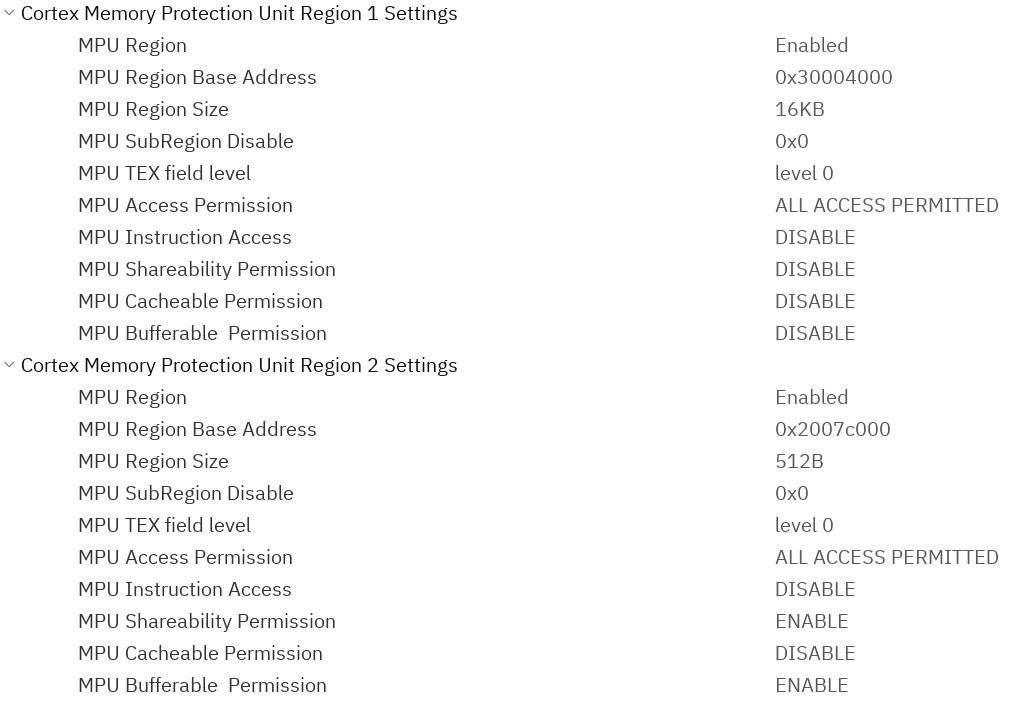
\includegraphics[width=1\textwidth]{assets/mpu_conf_cubemx}
    \caption{MPU-Konfiguration aus STM32CubeMX}
\end{figure}

Hierbei sind die Anfangsadressen sowie die Größe der RX- und TX-Deskriptoren
und des LwIP-Heaps aus CubeMX-Standardkonfigurationen entnommen.

Obwohl die MPU korrekt konfiguriert wurde, tritt dennoch ein Fehler auf, sobald
die Verbindung zum Micro-ROS-Client hergestellt wird. Der Fehler
(\ref{fig:micro_ros_err}) deutet darauf hin, dass bei der Datenübertragung über
UDP weiterhin Probleme auftreten. Insbesondere scheint das
\mintinline{text}|client_key| bzw. die assoziierten Daten immer noch nicht
ordentlich gecacht zu sein.

\begin{figure}[H]
    \centering
    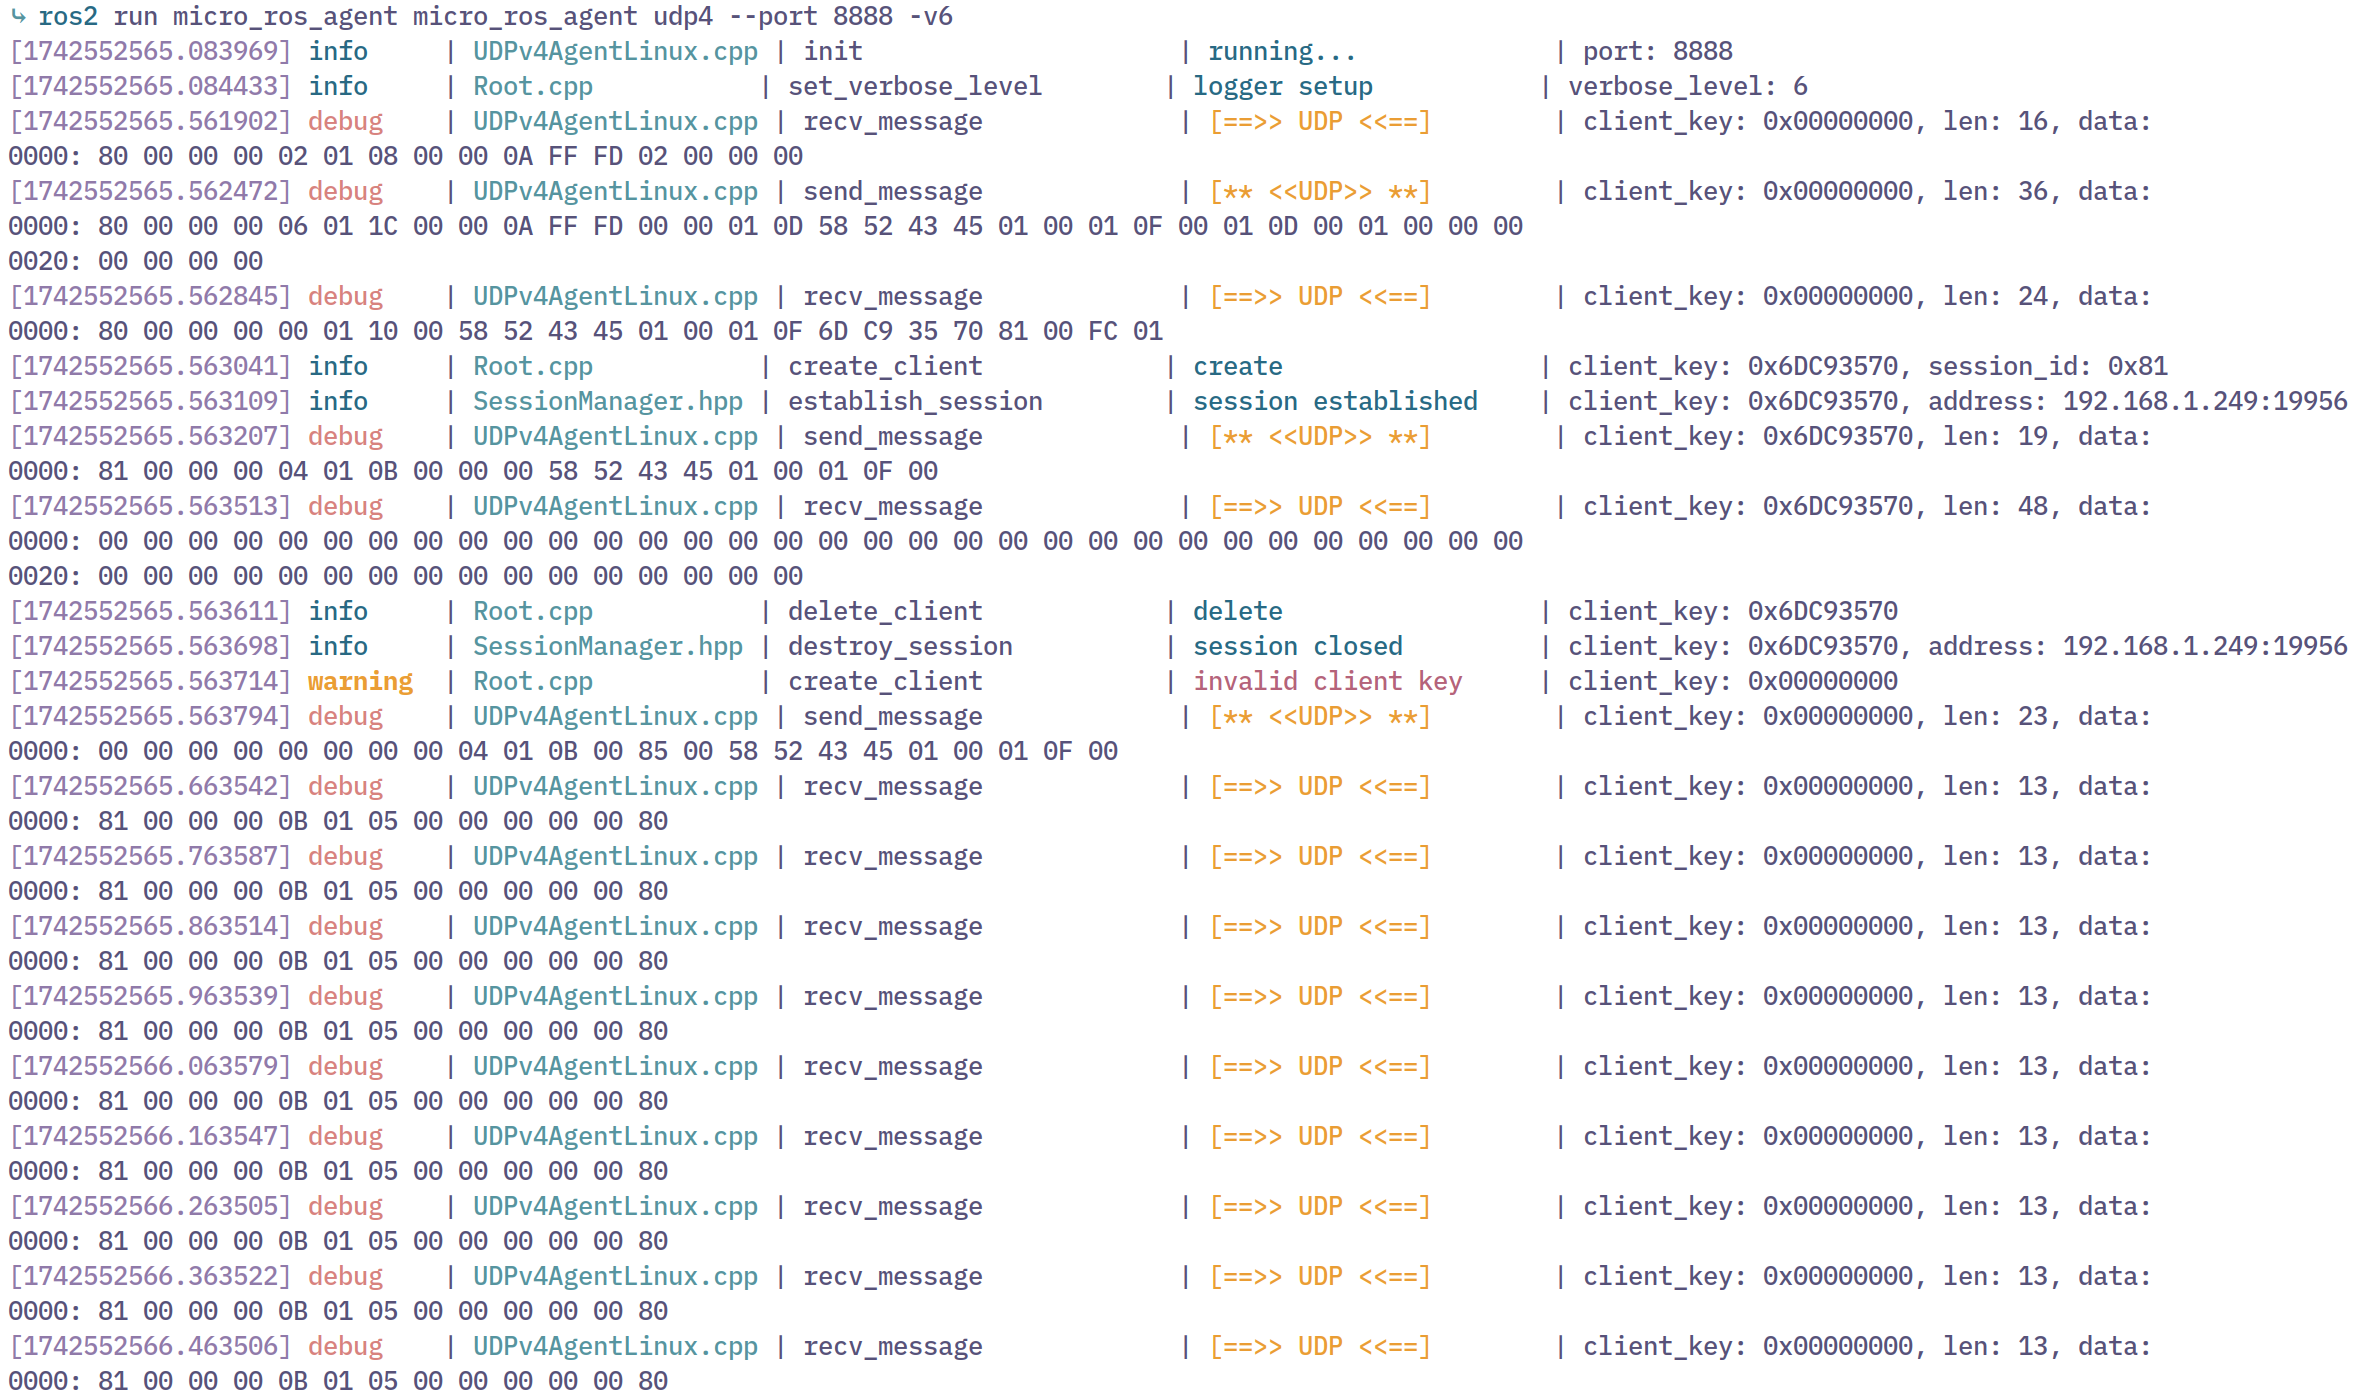
\includegraphics[width=1\textwidth]{assets/micro_ros_agent_err}
    \caption{Micro-ROS-Agent Debugausgaben}
    \label{fig:micro_ros_err}
\end{figure}

Bei der Recherche zu diesem Problem wurde ein Issue auf GitHub identifiziert
\cite{microROS_STM32CubeMX_Issue139}, welches genau dasselbe Verhalten
beschrieb. In diesem Kontext wurde dann der Autor um eine Lösung gebeten, die
daraufhin bereitgestellt wurde und sich als effektiv erwies, um das Problem zu
beheben.

\begin{code}
\begin{minted}{diff}
@@ -54,6 +54,10 @@
 /* USER CODE BEGIN 1 */
 /* address has to be aligned to 32 bytes */
+#define ALIGN_ADDR(addr) ((uintptr_t)(addr) & ~0x1F)
+#define ALIGN_SIZE(addr, size) ((size) + ((uintptr_t)(addr) & 0x1f))
+#define FLUSH_CACHE_BY_ADDR(addr, size) \
+  SCB_CleanDCache_by_Addr((uint32_t *)ALIGN_ADDR(addr), ALIGN_SIZE(addr, size))
 /* USER CODE END 1 */

 /* Private variables ---------------------------------------------------------*/
@@ -404,6 +408,8 @@
     Txbuffer[i].buffer = q->payload;
     Txbuffer[i].len = q->len;

+    FLUSH_CACHE_BY_ADDR(Txbuffer[i].buffer, Txbuffer[i].len);
+
     if(i>0)
     {
       Txbuffer[i-1].next = &Txbuffer[i];
\end{minted}
    \captionof{listing}{Modifizierung des ST-Treibercodes in Diffansicht
    \cite{microROS_STM32CubeMX_Issue139_code}}
    \label{code:cache_clean}
\end{code}

Die Lösung funktioniert folgendermaßen: Bei jeder Übertragung im Treibercode in
\mintinline{cpp}|low_level_output()| muss der Cache für jeden Paketpuffer durch
den Funktionsaufruf \mintinline{cpp}|SCB_CleanDCache_by_Addr()| geleert werden,
so dass Daten-Modifizierungen tatsächlich in den Speicher geschrieben und
folglich auch beim DMA-Controller korrekt widergespiegelt werden
(\ref{sec:cache_coherency}). Dieser Ansatz ist ebenfalls sowohl in einem Beitrag
aus dem Jahr 2018 im ST-Forum~\cite{ST_Forum_Post_2018}, als auch auf der
offiziellen LwIP-Webseite~\cite{lwip_pitfalls} dokumentiert.

Dabei muss die übergebene Speicheradresse durch eine bitweise UND-Verknüpfung
mit \mintinline{text}|~0x1F| auf eine 32-Byte-Grenze ausgerichtet
werden~\cite{CMSIS_Core_CacheFunctions}, indem die letzten 5 Bits gelöscht
werden. Nach der Anpassung der Adresse muss die Größe dementsprechend wieder
ergänzt werden, um die ausgegrenzten Bytes nach der Ausrichtung wieder zu
berücksichtigen.

Hierbei ist zu beachten, dass ein Teil der Modifizierung direkt im generierten
Treibercode vorgenommen wird, der bei nachfolgender Neugenerierung überschrieben
wird: In der Funktion \mintinline{cpp}|low_level_output()| ist kein durch ST
bereitgestellter Überschreibschutz für den User-Code vorhanden, und ein manuell
hinzugefügter Überschreibschutz ist ebenfalls unwirksam. Um dieses Problem zu
umgehen, wurde eine Patch-Datei erstellt, die nach jeder Neugenerierung auf die
entsprechende Datei \mintinline{text}|LWIP/Target/ethernetif.c| angewendet
werden muss.
